\documentclass[11pt,a4paper]{article}

\usepackage[utf8]{inputenc}
\usepackage[T1]{fontenc}
\usepackage[margin=1in]{geometry}
\usepackage{amsmath,amssymb,amsfonts}
\usepackage{graphicx}
\usepackage{xcolor}
\usepackage{booktabs}
\usepackage{tabularx}
\usepackage{array}
\usepackage{listings}
\usepackage{tikz}
\usetikzlibrary{shapes.geometric, arrows.meta, positioning, calc, fit}
\usepackage{enumitem}
\usepackage{caption}
\usepackage{subcaption}
\usepackage{float}
\usepackage{hyperref}

\hypersetup{
    colorlinks=true,
    linkcolor=black,
    citecolor=black,
    urlcolor=blue!70!black,
    pdftitle={Integrated Main Project: ARP + DHCP + Telnet},
    pdfauthor={Hrishikesh Bhanja, Aritra Dutta, Subham Bhat}
}

\definecolor{codebg}{rgb}{0.96,0.96,0.96}
\definecolor{codeframe}{rgb}{0.25,0.25,0.25}
\definecolor{codenum}{rgb}{0.45,0.45,0.45}

\lstset{
    backgroundcolor=\color{codebg},
    basicstyle=\ttfamily\footnotesize,
    breakatwhitespace=false,
    breaklines=true,
    captionpos=b,
    commentstyle=\color{codenum}\itshape,
    keywordstyle=\bfseries,
    numberstyle=\tiny\color{codenum},
    numbers=left,
    numbersep=8pt,
    frame=single,
    rulecolor=\color{codeframe},
    tabsize=4,
    columns=flexible,
    keepspaces=true,
    showspaces=false,
    showstringspaces=false,
    xleftmargin=14pt,
    xrightmargin=4pt,
    literate={→}{{$\rightarrow$}}1 {←}{{$\leftarrow$}}1 {–}{{--}}1 {—}{{---}}1 {·}{{$\cdot$}}1 {✓}{{OK}}2 {✗}{{X}}1
}

\newcolumntype{Y}{>{\raggedright\arraybackslash}X}

% screenshot from docs/screenshots (skipped quietly if the file is missing)
\newcommand{\shot}[3][0.92\textwidth]{%
  \IfFileExists{docs/screenshots/#2}{%
  \begin{figure}[H]\centering
  \includegraphics[width=#1,keepaspectratio]{docs/screenshots/#2}
  \caption{#3}\end{figure}}{}}

\emergencystretch=3em
\setlength{\parindent}{1.5em}
\setlength{\parskip}{0.4em}

\begin{document}

% ==============================================================================
% TITLE PAGE
% ==============================================================================
\begin{titlepage}
    \centering
    \vspace*{4.2cm}

    {\LARGE \textbf{One Campus LAN: Integrating ARP, DHCP}}\\[0.7em]
    {\LARGE \textbf{and Telnet with DHCP Snooping, ARP}}\\[0.7em]
    {\LARGE \textbf{Poisoning, and Dynamic ARP Inspection}}\\[1.4em]

    {\large for Computer Networks Laboratory}

    \vspace{3.8cm}

    {\large \textbf{Group members}}\\[0.8em]
    {\large
    \begin{tabular}{@{}ll@{}}
    Hrishikesh Bhanja & ARP module \\[0.35em]
    Aritra Dutta & DHCP module \\[0.35em]
    Subham Bhat & Telnet module and the integration \\
    \end{tabular}}\\[1.4em]
    {\large
    \textbf{Class:} BCSE III\\[0.55em]
    \textbf{Group:} A1\\[0.55em]
    \textbf{College:} Jadavpur University
    }

    \vfill
    {\normalsize 1}
\end{titlepage}

% ==============================================================================
% TABLE OF CONTENTS
% ==============================================================================
\pagenumbering{roman}
\setcounter{page}{2}
\tableofcontents
\newpage

% ==============================================================================
% MAIN CONTENT
% ==============================================================================
\pagenumbering{arabic}
\setcounter{page}{3}

\section{Introduction}
\noindent Our project basket is \textbf{ARP}, \textbf{DHCP} and \textbf{Telnet}. They are usually taught as three separate protocols at three different layers, yet a host joining a LAN needs all three, in order:
\begin{enumerate}[leftmargin=2em]
    \item an \textbf{IP address}, from DHCP (RFC 2131);
    \item the \textbf{MAC address of its next hop}, from ARP (RFC 826), after checking with ARP that its new address is not already in use (RFC 5227);
    \item a \textbf{management session} to the router, which on many campus networks is still Telnet (RFC 854).
\end{enumerate}
The three are also linked by security. ARP is unauthenticated, so an attacker can poison caches and redirect traffic. The most valuable traffic to steal is a Telnet login, which is clear text. The standard defence, \textbf{Dynamic ARP Inspection} (DAI), needs a trusted table of which MAC owns which IP, and that table is built by \textbf{DHCP snooping}. Finally, the administrator switches DAI on through the router's Telnet CLI.

The three modules were built separately by the members of Group A1: \textbf{ARP} by Hrishikesh Bhanja, \textbf{DHCP} by Aritra Dutta, and \textbf{Telnet} by Subham Bhat. This report describes the \textbf{integration}, written by Subham Bhat, in \texttt{MainProject}: one campus LAN, 192.168.1.0/24, on which the three modules run together and depend on one another, with a ten-step story that shows each dependency for real.

\subsection{What Was Built}
\begin{enumerate}[leftmargin=2em]
    \item \textbf{An integration bus} (\texttt{campus.Bus}) that starts the DHCP cluster and the ARP lab's switch with all hosts, and joins them only through the modules' public APIs.
    \item \textbf{DHCP $\rightarrow$ ARP}: every active lease becomes a DHCP-snooping binding on the switch; a declined lease removes it again.
    \item \textbf{ARP $\rightarrow$ DHCP}: an address conflict found by an ARP probe makes the client send a real DHCPDECLINE.
    \item \textbf{Telnet $\rightarrow$ ARP}: a relay carries every Telnet chunk as an Ethernet frame across the ARP lab's switch to the MAC address in the sender's ARP cache, so ARP poisoning really decides who receives the Telnet bytes.
    \item \textbf{Telnet $\rightarrow$ DHCP and ARP}: router CLI commands that show and change the other modules' tables and enable DAI.
    \item \textbf{A Packet Tracer--style dashboard} on \texttt{http://localhost:8089} that replays every packet each step produced, with a PDU panel and an event list.
    \item \textbf{18 end-to-end checks} (\texttt{run.bat --verify}).
\end{enumerate}

\shot{01_campus_start.png}{The campus LAN at the start of the story.}

% ==============================================================================
\section{The Campus Network}

\begin{table}[H]
\centering
\caption{Stations on switch CSE-Switch}
\small
\begin{tabularx}{\textwidth}{@{}llllY@{}}
\toprule
\textbf{Station} & \textbf{Port} & \textbf{IP} & \textbf{MAC} & \textbf{Role} \\ \midrule
Host-A & Fa0/1 & 192.168.1.10 (static) & \texttt{AA:AA:AA:11:11:11} & Causes the address conflict \\
Host-B & Fa0/2 & 192.168.1.20 (static) & \texttt{BB:BB:BB:22:22:22} & \\
Host-C & Fa0/3 & 192.168.1.30 (static) & \texttt{CC:CC:CC:33:33:33} & \\
JU-Main-R & Fa0/4 (trusted) & 192.168.1.1 & \texttt{00:1A:2B:00:01:01} & Gateway, DHCP relay, Telnet VTY lines \\
Kali-Attacker & Fa0/5 & 192.168.1.66 & \texttt{66:66:66:66:66:66} & ARP poisoning (man in the middle) \\
admin-laptop & Fa0/6 & from DHCP & \texttt{3C:52:82:AD:00:01} & The newcomer \\ \bottomrule
\end{tabularx}
\end{table}

\noindent The DHCP cluster (a load balancer on UDP 6700 with consistent hashing, and three nodes on 6701--6703) serves the pool 192.168.1.10--150 with gateway 192.168.1.1. The Telnet server listens on 2323 (TLS 9923); the relay that carries its bytes across the simulated LAN listens on 2325 (TLS 9925). The three modules' own dashboards stay available on 8080 (DHCP), 8081 (Telnet) and 8082 (ARP).

% ==============================================================================
\section{Integration Architecture}

\begin{figure}[H]
\centering
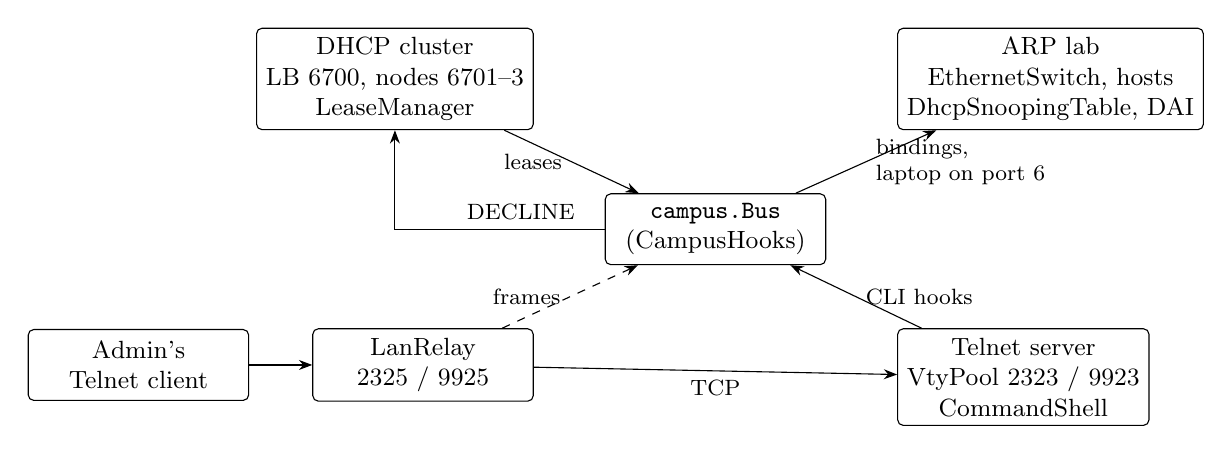
\begin{tikzpicture}[node distance=0.8cm, box/.style={draw, rounded corners=2pt, minimum width=2.8cm, minimum height=0.9cm, align=center, font=\small}, >=Stealth]
\node[box] (bus) {\texttt{campus.Bus}\\(CampusHooks)};
\node[box, above left=0.8cm and 0.9cm of bus] (dhcp) {DHCP cluster\\LB 6700, nodes 6701--3\\LeaseManager};
\node[box, above right=0.8cm and 0.9cm of bus] (arp) {ARP lab\\EthernetSwitch, hosts\\DhcpSnoopingTable, DAI};
\node[box, below right=0.8cm and 0.9cm of bus] (tel) {Telnet server\\VtyPool 2323 / 9923\\CommandShell};
\node[box, below left=0.8cm and 0.9cm of bus] (relay) {LanRelay\\2325 / 9925};
\node[box, left=0.8cm of relay] (cl) {Admin's\\Telnet client};
\draw[->] (dhcp) -- node[left, font=\footnotesize, align=right]{leases} (bus);
\draw[->] (bus) -- node[right, font=\footnotesize, align=left]{bindings,\\laptop on port 6} (arp);
\draw[->] (bus.west) -| node[above, pos=0.2, font=\footnotesize]{DECLINE} (dhcp.south);
\draw[->] (cl) -- (relay); \draw[->] (relay) -- node[below, font=\footnotesize]{TCP} (tel);
\draw[->, dashed] (relay) -- node[left, font=\footnotesize]{frames} (bus);
\draw[->] (tel) -- node[right, font=\footnotesize]{CLI hooks} (bus);
\end{tikzpicture}
\caption{How the three modules are joined.}
\end{figure}

\noindent \texttt{run.bat} compiles the three modules from their own folders together with the integration package:
\begin{lstlisting}[numbers=none]
javac --release 11 -encoding UTF-8 -d out ^
      -sourcepath "..\ARP\src;..\DHCP\src;..\Telnet\src;src" ^
      src\campus\*.java
\end{lstlisting}

\begin{table}[H]
\centering
\caption{Integration classes in \texttt{MainProject/src/campus}}
\small
\begin{tabularx}{\textwidth}{@{}lY@{}}
\toprule
\textbf{Class} & \textbf{Job} \\ \midrule
\texttt{Bus} & Starts the DHCP cluster and the switch with all hosts; syncs leases into the snooping table; runs the probe, decline and poisoning actions; implements \texttt{CampusHooks}. \\
\texttt{LanRelay} & Passes the real Telnet TCP session through and sends each chunk as an Ethernet frame across the switch. \\
\texttt{Recorder} & Captures what each step produced: DHCP log lines, frames seen at the switch, Telnet bytes decoded into NVT tokens. \\
\texttt{Story} & The ten steps; each \textbf{Forward} performs real protocol actions and returns the replay. \\
\texttt{Dashboard} & HTTP API (\texttt{/api/state}, \texttt{/api/forward}, \texttt{/api/restart}) and the page. \\
\texttt{Verify} & The end-to-end checks. \\ \bottomrule
\end{tabularx}
\end{table}

\noindent Only two changes were made outside \texttt{MainProject}: the Telnet module gained the \texttt{CampusHooks} interface and the router commands that use it, and a compile error in the ARP module's \texttt{Hub.java} was fixed.

% ==============================================================================
\section{Implementation of the Links}

\subsection{DHCP $\rightarrow$ ARP: Leases Become Snooping Bindings}
The bus reads every DHCP node's \texttt{LeaseManager}. Each ACTIVE lease is added to the switch's \texttt{DhcpSnoopingTable}. When a lease is DECLINED, its binding is removed and any static binding it had displaced (Host-A's, in the story) is restored.

\begin{lstlisting}[language=Java, caption={\texttt{Bus.syncLeases()}.}]
public synchronized void syncLeases() {
    for (DhcpServerNode n : nodes) for (LeaseRecord r : n.getLeaseManager().getAllLeases()) {
        String key = r.getIpAddress() + "|" + r.getMacAddress().toUpperCase();
        if (r.getState() == LeaseRecord.State.DECLINED && bound.removeIf(k -> k.startsWith(r.getIpAddress() + "|"))) {
            DhcpSnoopingTable.Binding old = displaced.remove(r.getIpAddress());
            if (old != null) snooping.addBinding(old.ip, old.mac, old.port, old.hostname);   // give .10 back to Host-A
            continue;
        }
        if (r.getState() != LeaseRecord.State.ACTIVE) continue;
        if (!bound.add(key)) continue;                                     // already bound
        int port = r.getMacAddress().equalsIgnoreCase(ADMIN_MAC) ? ADMIN_PORT : 0;
        IpAddress lip = IpAddress.parse(r.getIpAddress());
        DhcpSnoopingTable.Binding prev = snooping.getBinding(lip);
        if (prev != null && !prev.mac.equals(MacAddress.parse(r.getMacAddress()))) displaced.put(r.getIpAddress(), prev);
        snooping.addBinding(lip, MacAddress.parse(r.getMacAddress()), port, r.getHostname());
    }
}
\end{lstlisting}

\subsection{ARP $\rightarrow$ DHCP: Conflict Detection and DHCPDECLINE}
After DORA the laptop probes its new address with an ARP request whose sender IP is 0.0.0.0 (RFC 5227). Host-A owns .10 and defends it with a gratuitous ARP. The bus detects the defence and calls the DHCP client's \texttt{sendDecline}, which sends a real DHCPDECLINE over UDP; the cluster marks the address as declined and the second DORA yields .11.

\subsection{Telnet $\rightarrow$ ARP: Telnet Bytes as Frames on the Switch}
\texttt{LanRelay} forwards the real TCP session between the admin's client and the Telnet server. For every chunk it also asks the bus to send an IPv4 frame from the sender's network interface to the MAC address that the sender's ARP cache holds for the destination IP. When the cache is clean, the frame reaches the router's port; when it is poisoned, it reaches the attacker's port, and the attacker's frame handler logs the Telnet text.

\begin{lstlisting}[language=Java, caption={\texttt{Bus.telnetBytes()}: who receives the Telnet chunk is decided by ARP.}]
public void telnetBytes(boolean toRouter, byte[] b, int n, boolean tls) {
    String text = tls ? "TLS record, " + n + " bytes (encrypted)" : printable(b, n);
    String payload = "TELNET " + (toRouter ? ip + " > " + GATEWAY + ":23" : GATEWAY + ":23 > " + ip) + " | " + text;
    HostNode from = toRouter ? admin : router;
    IpAddress dst = toRouter ? router.getNic().getIp() : IpAddress.parse(ip);
    MacAddress mac = from.getArpTable().lookupMac(dst);                  // ask the sender's ARP cache
    if (mac == null) { from.sendArpRequest(dst); mac = from.getArpTable().lookupMac(dst); }
    if (mac == null) return;
    int toPort = mac.equals(attacker.getNic().getMac()) ? 5 : toRouter ? 4 : ADMIN_PORT;
    rec.telnet(toRouter, b, n, tls, toPort, ip);                         // for the replay
    from.getNic().send(new EthernetFrame(mac, from.getNic().getMac(),
            EthernetFrame.ETHERTYPE_IPV4, payload.getBytes(StandardCharsets.UTF_8)));
}
\end{lstlisting}

\subsection{Telnet $\rightarrow$ DHCP and ARP: Router Commands}
The Telnet server's \texttt{CommandShell} calls the bus through \texttt{CampusHooks}:
\begin{itemize}[leftmargin=2em]
    \item \texttt{show ip dhcp binding}: the live leases from the DHCP cluster;
    \item \texttt{show ip arp}, \texttt{show mac address-table}: the router's ARP cache and the switch's CAM table;
    \item \texttt{show ip arp inspection}, \texttt{clear arp-cache};
    \item \texttt{ip arp inspection vlan 1} and \texttt{no ip arp inspection vlan 1} in configuration mode: switch DAI on or off.
\end{itemize}

\subsection{The Replay}
After each step, \texttt{Recorder} returns the packets it produced. The dashboard animates them on a Packet Tracer--style topology:
\begin{itemize}[leftmargin=2em]
    \item a DHCP DISCOVER or REQUEST fans out to every port (PCs drop it with \texttt{X}; the router relays it to the load balancer, which hashes the MAC to one node);
    \item an ARP request floods every port (\texttt{OK} at the owner) and the reply returns as unicast;
    \item a Telnet segment walks down the laptop's stack (terminal, terminal driver, Telnet client and NVT, TCP, IP, Ethernet) and up the router's to the \textbf{pseudo-terminal driver} and the shell, showing the real NVT bytes, for example \texttt{IAC DO ECHO} = \texttt{FF FD 01}. The bytes also ride under the envelope as it crosses the topology: one cell per byte with its name, its 8 bits and its hex value, control bytes (most significant bit 1) in dark red and data bytes (most significant bit 0) in light colour, so the password can be watched travelling one character per segment.
\end{itemize}

\shot{07_dhcp_discover_broadcast.png}{DHCP DISCOVER as a layer-2 broadcast, relayed to the cluster.}

% ==============================================================================
\section{The Story and Its Results}
Each press of \textbf{Forward} runs one step for real. The outcomes below are those produced by the module.

\begin{table}[H]
\centering
\caption{The ten steps}
\small
\begin{tabularx}{\textwidth}{@{}clY@{}}
\toprule
\textbf{\#} & \textbf{Step} & \textbf{What happens} \\ \midrule
1 & A laptop asks for an address & Real DORA over UDP; the cluster offers 192.168.1.10. \\
2 & Is that address really free? & ARP probe (sender IP 0.0.0.0); Host-A defends .10 with a gratuitous ARP; the laptop sends DHCPDECLINE. Host-A's snooping binding is restored. \\
3 & Second lease, clean probe & DORA again gives .11; the probe gets no answer; gratuitous ARP; the binding .11 $\leftrightarrow$ laptop on port 6 appears in the snooping table. \\
4 & Find the gateway & ARP request for 192.168.1.1 floods the switch; the router replies by unicast; the laptop's cache and the switch's CAM table fill in. \\
5 & The admin telnets into the router & Login as \texttt{admin}; \texttt{show ip dhcp binding} and \texttt{show ip arp} print the live tables of the other two modules. \\
6 & An attacker poisons the ARP caches & Forged ARP replies (inspection is off): the laptop now maps 192.168.1.1 to the attacker's MAC; the path is drawn in red. \\
7 & The next login is sniffed & The Telnet frames go to port 5; the attacker's notebook shows \texttt{admin} / \texttt{cisco}. \\
8 & Fix it from the router & \texttt{ip arp inspection vlan 1} typed in the same Telnet session switches DAI on. \\
9 & Log in again: nothing leaks & The forged replies are dropped at the switch port because no DHCP binding supports them; the login reaches the router; the notebook stays empty. \\
10 & Defence in depth: Telnet over TLS & With inspection off and the LAN poisoned again, the session runs over TLS; the attacker sees only encrypted records. \\ \bottomrule
\end{tabularx}
\end{table}

\shot{02_dhcp_decline.png}{Step 2: the ARP probe finds Host-A on .10 and the laptop declines the lease.}
\shot{04_password_sniffed.png}{Step 7: after ARP poisoning, the attacker reads the Telnet credentials.}
\shot{05_dai_blocks_attack.png}{Step 9: with DAI on, the forged ARP replies are dropped using the DHCP bindings.}
\shot{09_telnet_stack_pty.png}{A Telnet segment walking up the router's stack to the pseudo-terminal driver.}

\subsection{Running and Verification}
\begin{lstlisting}[language=bash, caption={Running the integrated project.}]
cd MainProject
run.bat                  # compiles ARP + DHCP + Telnet + campus; story at http://localhost:8089
run.bat --verify         # 18 end-to-end checks
telnet 127.0.0.1 2325    # a Telnet session across the simulated LAN (admin / cisco)
\end{lstlisting}

\begin{table}[H]
\centering
\caption{End-to-end checks (all passed)}
\small
\begin{tabularx}{\textwidth}{@{}Y@{}}
\toprule
Real DORA over UDP: the cluster leases 192.168.1.10 to the laptop \\
ARP $\rightarrow$ DHCP: the probe finds Host-A on .10 and the client sends DHCPDECLINE \\
After the decline, .10's snooping binding is Host-A's again; the second lease is a different, conflict-free address \\
DHCP $\rightarrow$ ARP: the lease is in the switch's DHCP-snooping table \\
The laptop's ARP cache maps 192.168.1.1 to the router's MAC; the switch learned the laptop's MAC on port 6 \\
Telnet $\rightarrow$ DHCP: \texttt{show ip dhcp binding} lists the live lease; Telnet $\rightarrow$ ARP: \texttt{show ip arp} lists the laptop \\
No interception before the attack; ARP poisoning succeeds while inspection is off \\
ARP $\rightarrow$ Telnet: the attacker reads the Telnet user name and password \\
Telnet $\rightarrow$ ARP: \texttt{ip arp inspection vlan 1} typed on the router enables DAI; forged replies are dropped using the DHCP bindings \\
The next Telnet login is not intercepted; on a poisoned LAN a TLS session leaks only encrypted records \\
After Restart the story begins again from an empty lease database \\ \bottomrule
\end{tabularx}
\end{table}

% ==============================================================================
\section{Conclusion}
\begin{enumerate}[leftmargin=2em]
    \item \textbf{The three protocols depend on each other.} DHCP supplies the address and the trusted bindings, ARP checks the address and resolves the gateway, and Telnet manages the router. Integrating the modules made each dependency visible as a real message: a DHCPDECLINE caused by an ARP probe, and a snooping binding created by a DHCP ACK.
    \item \textbf{A weakness in one layer breaks another.} Because ARP accepts unsolicited replies, poisoning redirected real Telnet bytes to the attacker, who read the clear-text password.
    \item \textbf{The fix comes from a third protocol.} Dynamic ARP Inspection, using the bindings that DHCP snooping built and enabled from the Telnet CLI, dropped the forged replies; Telnet over TLS protected the login even when inspection was off. Layered defences are needed because each one alone can be misconfigured.
\end{enumerate}

\section*{AI Acknowledgement}
\addcontentsline{toc}{section}{AI Acknowledgement}
Artificial Intelligence tools were used as an aid during this project. Specifically, AI assistance was used for:
\begin{itemize}[leftmargin=2em]
    \item \textbf{Protocol cross-checking:} comparing message formats, reply codes, state machines and byte offsets against the RFCs cited in this report.
    \item \textbf{Code review and testing:} suggesting edge cases for the automated verification suite and reviewing concurrency and error handling.
    \item \textbf{Writing and visualization:} drafting, structuring and refining the explanations, tables, diagrams and \LaTeX{} source of this report.
\end{itemize}
All protocol implementations, Java source code, experiments, measurements and final conclusions were run, reviewed and verified by the author, who takes full responsibility for the content of this report.

\end{document}
